\documentclass[12pt]{article}

\usepackage[margin=1in]{geometry}
\usepackage{xcolor}
\usepackage{setspace}
\usepackage{hyperref}
\usepackage{graphicx}
\usepackage{pgfplots}
\pgfplotsset{compat=1.18}

\setstretch{1.15}

\title{Coach Follow Up: \\ LLM-Assisted Conversation Evaluation}
\author{{Paul Becker, Zander Henson, Alan Villagrand, Ayo Adu, Giana Grace} \\
	School of Engineering and Computer Science, Baylor University}
\date{{May 8, 2026}}

\begin{document}
	
	\maketitle
	
	\section{Introduction -- Purpose}
	
	The purpose of this project is to design and implement a secure, usable, and extensible system for reviewing coaching conversations and surfacing high-priority follow-up opportunities. The application supports human reviewers by organizing conversations into a structured dashboard, highlighting relevant transcript snippets, attaching evaluation tags, and enabling review actions such as status updates, reviewer notes, and false-tag feedback. The system is intended to reduce manual review burden while preserving human oversight over sensitive or high-impact decisions.
	
	This project is best understood as a full-stack review platform with three tightly connected goals. First, it must present conversation data in a way that makes review efficient and understandable. Second, it must support a real operational workflow rather than simply displaying model output. Third, it must provide a path for integrating large language model (LLM) evaluation in a way that is technically practical, cost-conscious, and auditable.
	
	The resulting system includes a modern frontend for reviewing conversations, a backend built around Azure Functions and Azure SQL, and a data model that supports both machine-generated tags and human feedback. The platform also includes reporting features, authentication, and several workflow improvements that make it more suitable for ongoing production use.
	
	\section{Background and Problem Context}
	
	The central problem addressed by this project is that reviewing large numbers of coaching conversations manually is time-consuming and difficult to scale. If every conversation must be read in full by a human reviewer, then both the cost and time required for quality assurance become substantial. At the same time, fully automating review is not appropriate, because the output may contain ambiguities, edge cases, or false positives that still require human judgment.
	
	This creates a need for a hybrid system. LLM-based evaluation can be used to identify potentially important patterns, assign tags, and estimate priority. However, human reviewers must still be able to inspect the evidence, correct mistakes, and document their own judgments. In practice, this means the software must do more than display machine output. It must support an actual review workflow with review status, reviewer notes, transcript inspection, and analytics.
	
	The platform therefore evolved beyond a simple conversation viewer. It became a review environment in which machine evaluation is one input, but the final operational process remains human-guided.
	
	\section{System Overview}
	
	The system is composed of a frontend application, a backend API layer, a SQL database, blob-stored transcript data, and an LLM-assisted evaluation pipeline.
	
	The frontend is responsible for rendering the dashboard, transcript views, tag-management pages, pipeline administration views, reporting views, and authenticated user experience. The backend provides APIs for retrieving conversations, tags, tagged messages, transcript data, review metadata, and reporting aggregates. Azure SQL stores structured application data such as conversations, tags, tag definitions, review status, review notes, and false-tag feedback. Blob storage is used for full transcript content. The LLM pipeline produces machine-evaluated outputs that are then surfaced in the dashboard for human review.
	
	This architecture was chosen to preserve a clean separation of responsibilities. The frontend emphasizes usability and review workflow. The backend allows persistence, filtering, aggregation, and integration with storage systems. The evaluation pipeline remains logically separate so that model decisions and review tooling can evolve without tightly coupling every change to the web interface.
	
	\section{Frontend Architecture and Design Decisions}
	
	\subsection{Frontend Framework and Structure}
	
	The frontend was built in Next.js with TypeScript. This was a strong fit for the project because it supports server-rendered and client-rendered patterns in the same application, works well with route-based organization, and allows shared type definitions across features. The frontend codebase was organized into feature-specific modules such as dashboard, tags, reports, and pipeline administration. This made it easier to evolve each part of the application independently while preserving a consistent user experience.
	
	A major frontend design decision was to treat the dashboard not as a static reporting page, but as an operational workspace. As a result, the dashboard includes structured filters, conversation selection, transcript viewing, review status controls, reviewer notes, tag displays, and full conversation inspection. This approach was more useful than simply listing model-generated outputs because it supports the actual tasks a reviewer needs to perform.
	
	\subsection{Dashboard Workflow and Human Review Features}
	
	Several frontend decisions were driven by reviewer workflow rather than purely technical concerns. Review status was separated from evaluation status so that conversations are not mistakenly treated as human-reviewed simply because automated processing finished. Reviewer notes were added as a first-class feature so that reviewers can preserve context and follow-up reasoning. The full transcript view was implemented in a modal to make large conversations easier to inspect.
	
	Another important workflow decision was the addition of false-tag feedback. Each applied tag in a conversation can be marked as false, and a reviewer can attach a required note explaining why that tag was incorrectly applied. This preserves the machine output for auditability while also capturing human disagreement in a structured form. That decision is especially important for future evaluation quality analysis.
	
	\subsection{Filtering, Pagination, and Transcript Usability}
	
	The frontend also required careful handling of filtering and navigation for large conversation lists. Date-based filtering was added to support operational review windows such as today, the past two days, the past week, and all time. Pagination and infinite scrolling behavior were refined to prevent list-reset bugs and preserve a stable user experience when selecting items after loading additional pages. Transcript ordering and highlighting logic were also corrected so that the user sees the full conversation in proper chronological order while still being able to identify the specific messages associated with machine-generated tags.
	
	These decisions may appear small individually, but together they determine whether the system feels reliable enough for real review work.
	
	\section{Backend Architecture and Data Decisions}
	
	\subsection{Backend Framework and Storage}
	
	The backend was implemented using Python Azure Functions. This was a logical choice because it integrates naturally with other Azure services, including Azure SQL and Azure Blob Storage, and provides an serverless way to expose function-based APIs for the frontend, which reduces cost in the long-run.
	
	The database stores several different categories of information:
	\begin{itemize}
		\item conversation-level metadata
		\item tag definitions used by the evaluation system
		\item applied tags for specific conversations
		\item tagged messages associated with each applied tag
		\item human review status and review notes
		\item false-tag reviewer feedback
		\item reporting and pipeline support data
	\end{itemize}
	
	Blob storage is used for transcript payloads so that the full message content does not need to be duplicated inefficiently in every relational query path. Our ER diagram for the database is shown in figure 1.

    \begin{figure}
        \centering
        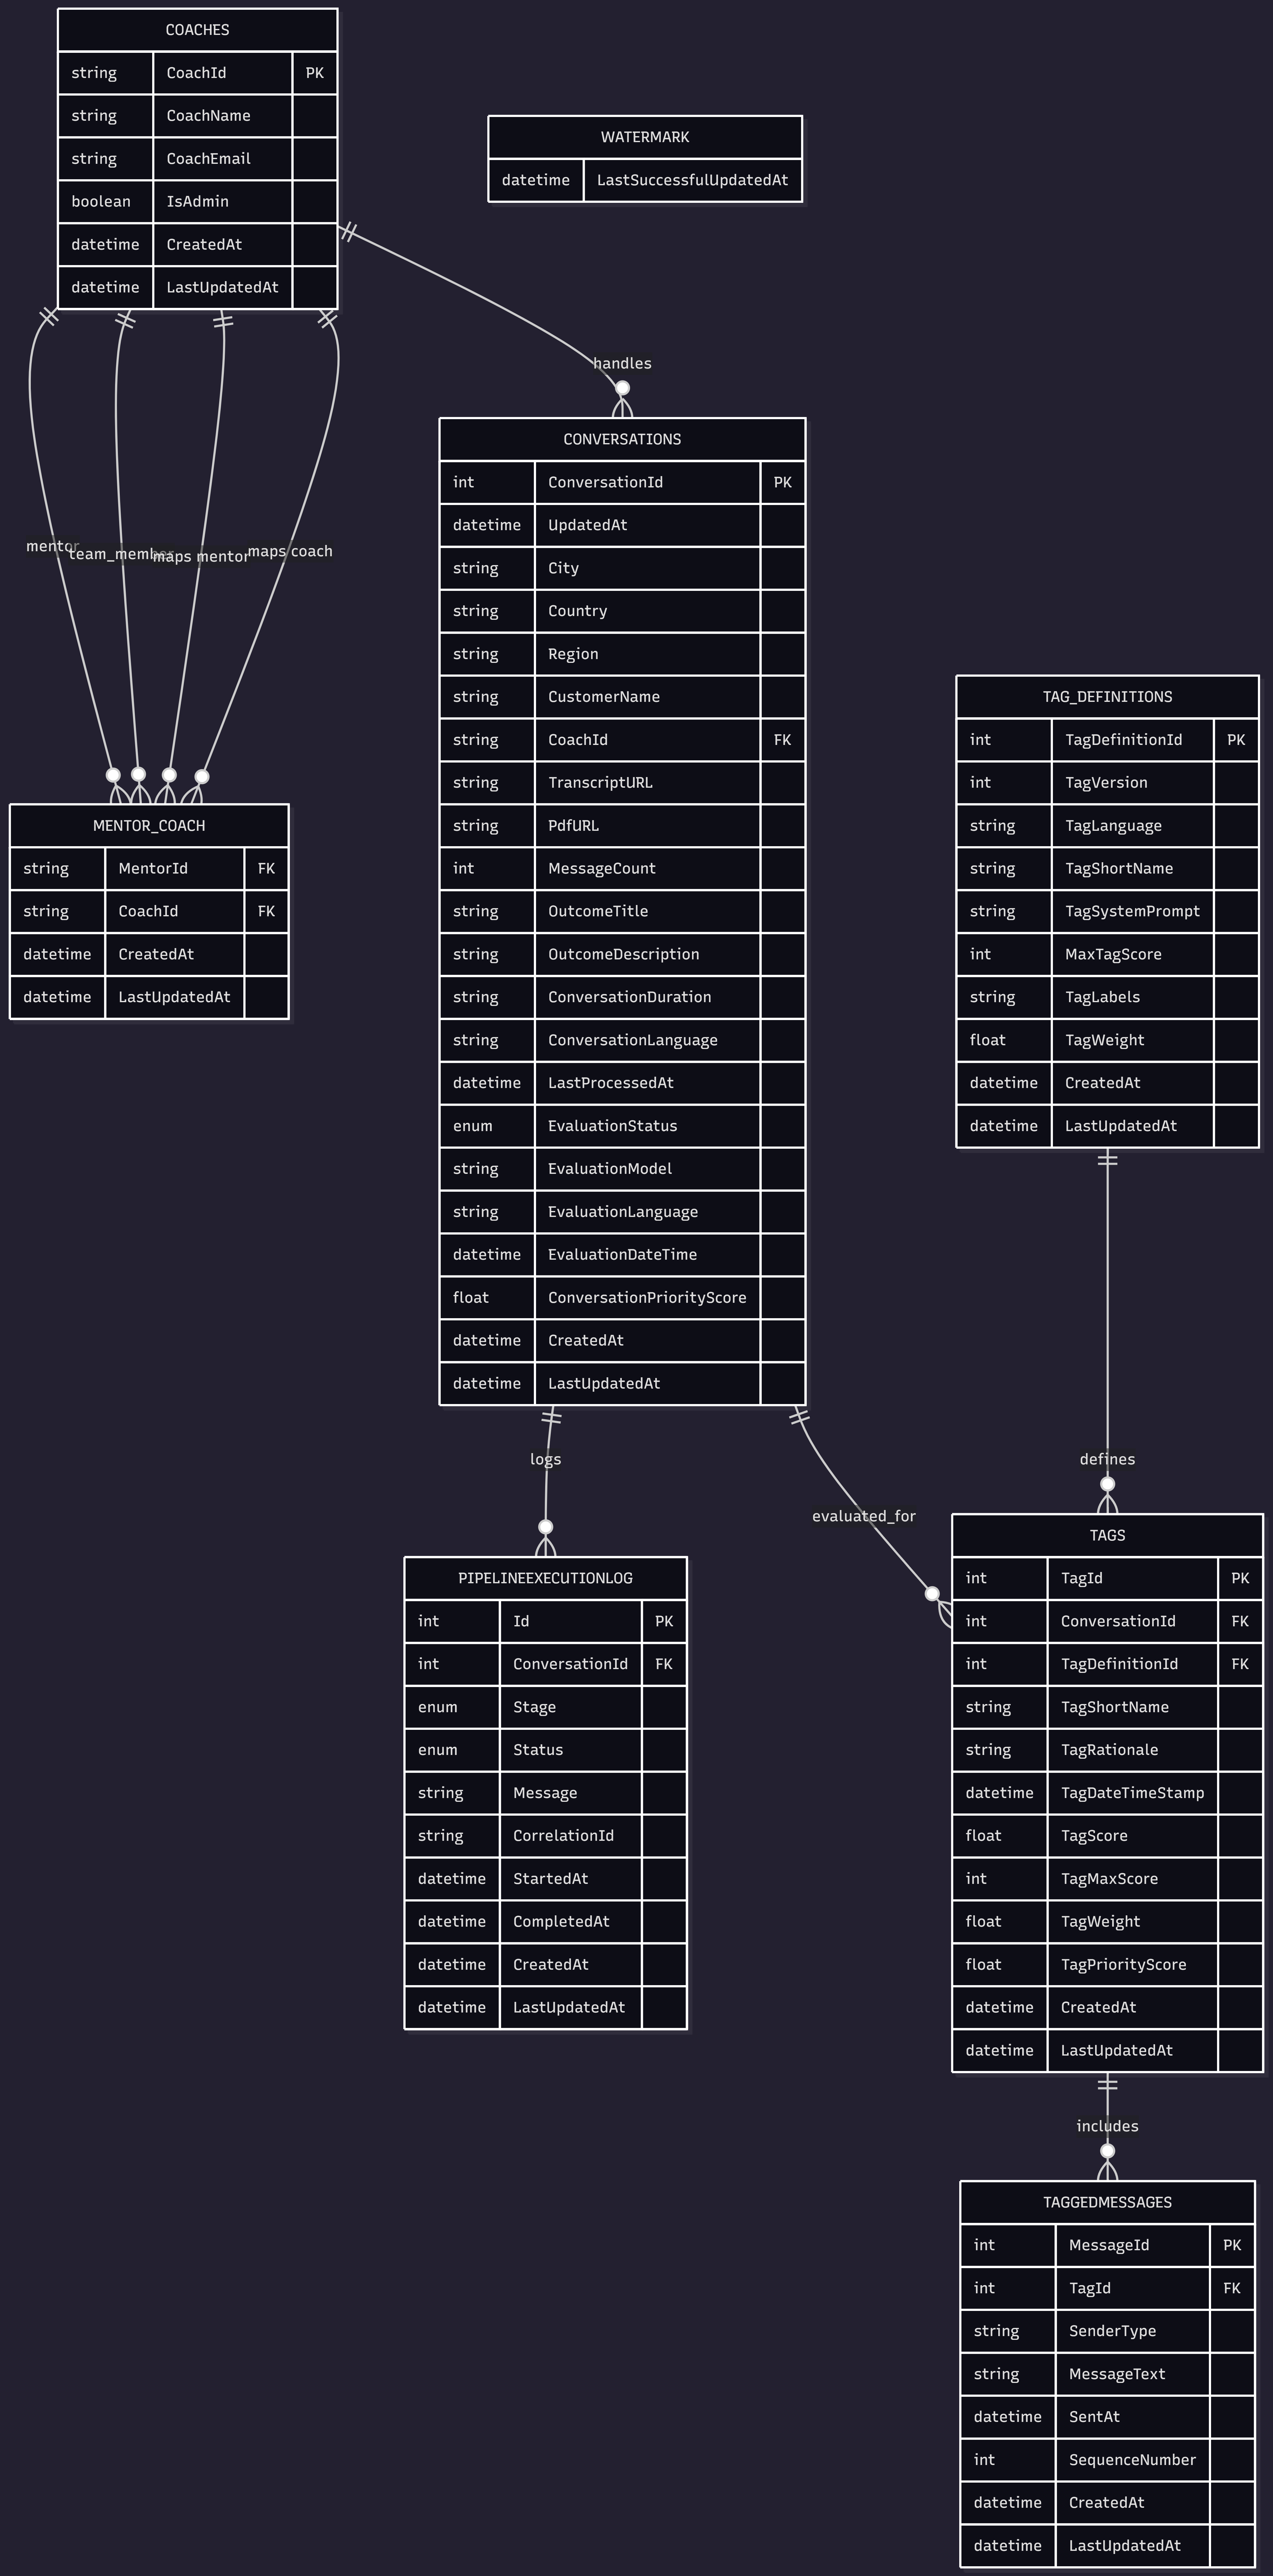
\includegraphics[width=0.5\linewidth]{er-diagram.png}
        \caption{Database ER diagram}
        \label{fig:er-diagram}
    \end{figure}

    \subsection{Backend Processing Pipeline and Queue Architecture}
    The core data processing pipeline is implemented as a multi-stage, queue-driven system using Azure Queue Storage to decouple ingestion from evaluation. This design ensures that failures in one stage do not cascade and that each conversation can be retried independently.
    
    The pipeline consists of two Azure Queue Storage queues and three logical stages per conversation:
    \paragraph{Queues.}
    \begin{itemize}
        \item \textbf{echo-etl-queue} -- Receives messages from a scheduled data fetch function (\texttt{ScheduledEchoDetch}) that runs daily at 1 AM CT. Each message contains a \texttt{conversationId}, a \texttt{stagingPath} pointing to a blob in Azure Blob Storage, and a \texttt{correlationId} for traceability. This queue is consumed by the \texttt{ProcessStagingMessage} function.
        
        \item \textbf{evaluation-queue} -- Receives messages after staging is complete. Each message contains a \texttt{conversationId} and \texttt{correlationId}. This queue is consumed by the \texttt{EvaluateConversation} function, which performs the LLM-based tag evaluation.
    \end{itemize}
    
    \paragraph{Pipeline Stages.} Each conversation progresses through three tracked stages, logged to the \texttt{PIPELINEEXECUTIONLOG} table:
    
    \begin{enumerate}
        \item \textbf{INGESTION} -- Triggered when \texttt{ProcessStagingMessage} dequeues an ETL message. The function reads the conversation payload from the staging blob, upserts metadata into the \texttt{CONVERSATIONS} table, copies the transcript to the canonical blob container, and enqueues a message to \texttt{evaluation-queue}. The conversation's \texttt{EvaluationStatus} is set to \texttt{PROCESSING}.
        
        \item \textbf{EVALUATION} -- Triggered when \texttt{EvaluateConversation} dequeues an evaluation message. The function retrieves the canonical transcript blob, constructs a prompt using tag definitions from \texttt{TAG\_DEFINITIONS}, and sends the conversation to Azure AI Foundry for tag scoring. The raw LLM response is parsed, and scores are normalized against tag definitions.
        
        \item \textbf{FINALIZATION} -- Persists evaluation results to SQL. Tag records are inserted into \texttt{TAGS} with computed priority scores, and supporting message evidence is inserted into \texttt{TAGGEDMESSAGES}. The conversation's \texttt{EvaluationStatus} is set to \texttt{COMPLETED} and \texttt{ReviewStatus} defaults to \texttt{NEEDS\_REVIEW}.
    \end{enumerate}
    
    \paragraph{Error Handling and Retry Behavior.} Azure Queue Storage provides automatic retry with configurable visibility timeout. If a function throws an unhandled exception, the message becomes visible again after the timeout expires. After exceeding the maximum dequeue count, the message is moved to the poison queue.
    Additionally, the pipeline logs status transitions (\texttt{IN\_PROGRESS}, \texttt{COMPLETED}, \texttt{FAILED}) for each stage in \texttt{PIPELINEEXECUTIONLOG}. On failure, all in-progress stages are marked \texttt{FAILED} and the conversation's \texttt{EvaluationStatus} is set to \texttt{FAILED}, allowing operators to identify and reprocess failed conversations through the pipeline stats API.
    \paragraph{Pipeline Orchestration.} The pipeline is triggered via timer trigger (\texttt{ScheduledEchoFetch}) that runs daily at 1 AM CT. The function syncs coach data from Echo, fetches yesterday's conversations, uploads each to staging blob storage, and enqueues ETL messages. A watermark (\texttt{PIPELINEWATERMARK} table) tracks the last successful run timestamp to prevent duplicate processing.
    \paragraph{Blob Storage Layout.}
    
    \begin{itemize}
        \item \textbf{staging/} -- Temporary location for raw conversation payloads fetched from Echo, organized by date (\texttt{staging/conversations/YYYY/MM/DD/\{id\}.json}).
        
        \item \textbf{canonical/} -- Permanent storage for processed transcripts (\texttt{canonical/conversations/YYYY/MM/DD/\{id\}.json}). The \texttt{TranscriptURL} in the \texttt{CONVERSATIONS} table references blobs in this container.
    \end{itemize}

    An overview of the system architecture is shown in Figure 2.

    \begin{figure}
        \centering
        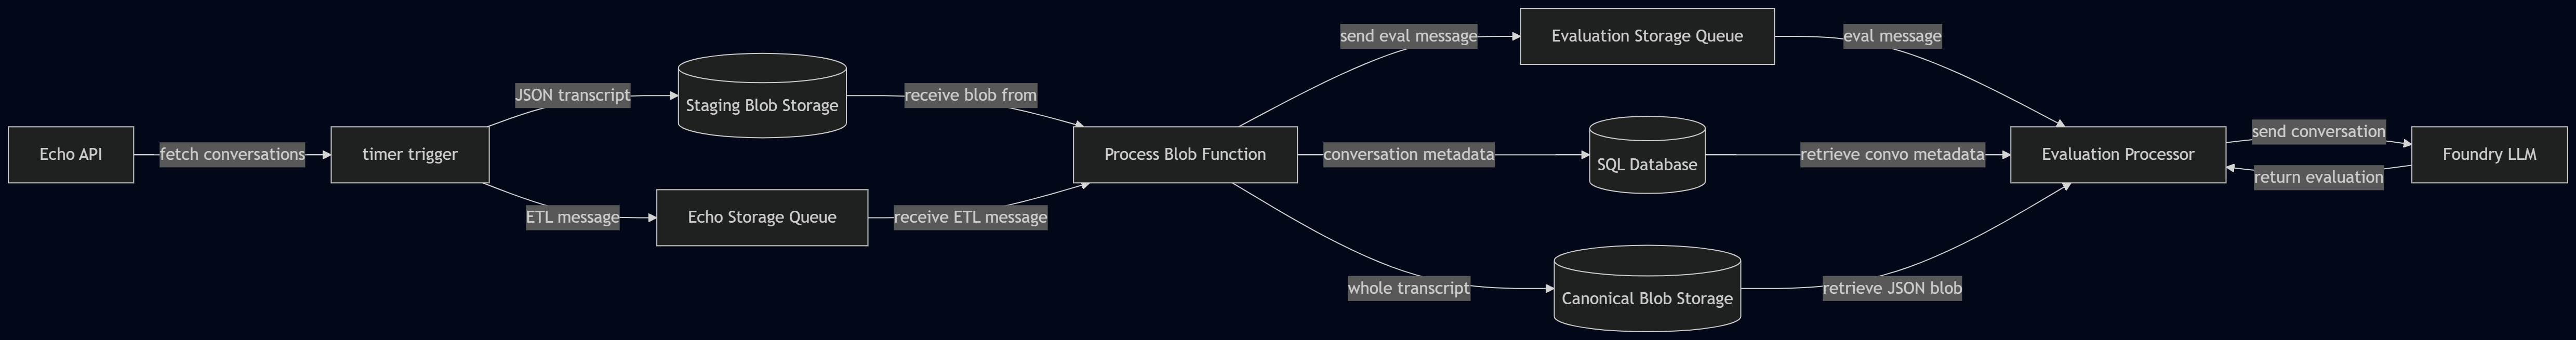
\includegraphics[width= \linewidth]{backend-architecture.png}
        \caption{System Architecture}
        \label{fig:backend-architecture}
    \end{figure}
    
	\subsection{Review Workflow Data Model}
	
	A key backend design decision was to separate machine-evaluation fields from human-review fields. Review status and reviewer notes are not the same as evaluation completion state, and the schema was adjusted to reflect that distinction. This improves clarity and prevents misleading UI behavior.
	
	Similarly, false-tag feedback was stored at the level of the applied tag within a conversation rather than at the tag-definition level. This is important because a tag definition may be valid in general while still being incorrectly applied to a specific conversation. The backend therefore needed to support a false flag, false-tag note, and false-tag timestamp on conversation-specific tag records.
	
	\subsection{Reporting and Aggregation Decisions}
	
	Reporting was implemented by aggregating existing SQL data rather than introducing a separate analytics database immediately. This was a pragmatic decision. The reports feature mainly needed tag counts and conversation-rate statistics across time buckets, so SQL-based aggregation was sufficient for the first version. This reduced implementation complexity while still supporting a useful reporting interface.
	
	The backend therefore became responsible for aggregation logic, date-range filtering, and trend computation, allowing the frontend to focus on rendering charts and controls rather than computing analytics itself.
	
	\section{Authentication and Security Design}
	
	The application uses Azure Static Web Apps authentication with Google. On the frontend, this includes a localized login page, route protection, redirect handling, logout support, and user context in the application shell. Local development uses the Azure Static Web Apps emulator, including a mock local-auth path for easier testing.
	
	This work secured the frontend session flow, but on the backend, requests pass through Static Web Apps so that the authenticated client principal can be injected into backend API requests. The backend can then validate the principal, restrict access to approved users, and later support role-based permissions if needed.
	
	\section{LLM Evaluation Architecture}
	
	\subsection{Why LLM Assistance Was Used}
	
	The role of the LLM layer in this project is to help identify potentially important patterns in coaching conversations, assign tags, and prioritize conversations for follow-up review. The LLM is not intended to replace human judgment. Instead, it is intended to reduce the amount of raw reading required and make human reviewers more effective by surfacing likely areas of concern.
	
	This design choice reflects an important practical principle: for a system involving nuanced interpersonal conversations, the most useful role for an LLM is often triage and structured assistance rather than final autonomous decision-making.
	
	\subsection{Model Selection, Prompting, Fine-Tuning, and Cost Tradeoffs}

    To begin with, we used Openrouter to quickly switch between different models. Early on, we made the key decision to use PromptFoo, an existing LLM evaluation framework. Combining these two technologies, were were rapidly able to experiment with different models, prompts, and evaluation prompts, all on real conversation data. 

    We first tried a very cheap model, MiniMax M2.5, with \$0.15/M input tokens \$1.15/M output tokens. 
    This helped us solidify a workable evaluation loop. 

    At this point, we also had our first prompt version, which integrated stakeholder feedback. 
    It had 10 tags, all in english, which were suggested by expert feedback from coaches. 
    The small models (gpt-4o-mini and MiniMax M2.5) were performing significantly worse, even on small samples. 
    Accuracies were as low as 46.67\% (7/15 conversations succesfully tagged). 
    However, a midrange model (Z.ai: GLM 5 Turbo) with \$1.20/M input tokens \$4/M output tokens was performing much better, with 85.71\% passing (12/14).

    We then tried a very expensive model to test the feasibility of LLM-evaluations. 
    Namely, we used claude-sonnet-4.6 at \$3/M input tokens and \$15/M output tokens.
    Even with our naive first prompt, the model had great performance, with 100\% accuracy on a small sample (14/14).

    Eventually, due to model constraints with Microsoft Foundry and cost constraints, we settled on gpt-5-mini (\$0.25/M input token \$2/M output tokens).
    To improve the prompt, we included example conversation flags derived from the output of previous experimentation and expert feedback. This allowed us to reach very high accuracy, 90.98\% passing (363/399 cases). 
    Furthermore, we used an AI prompt refiner, and scored an even higher accuracy, on an even bigger sample 95.30\% passing (1603/1682 cases). 
    Our experiments demonstrated that through prompt refinement, lower cost models can perform exceptionally on narrow tasks.

    \begin{figure}[htbp]
        \centering
        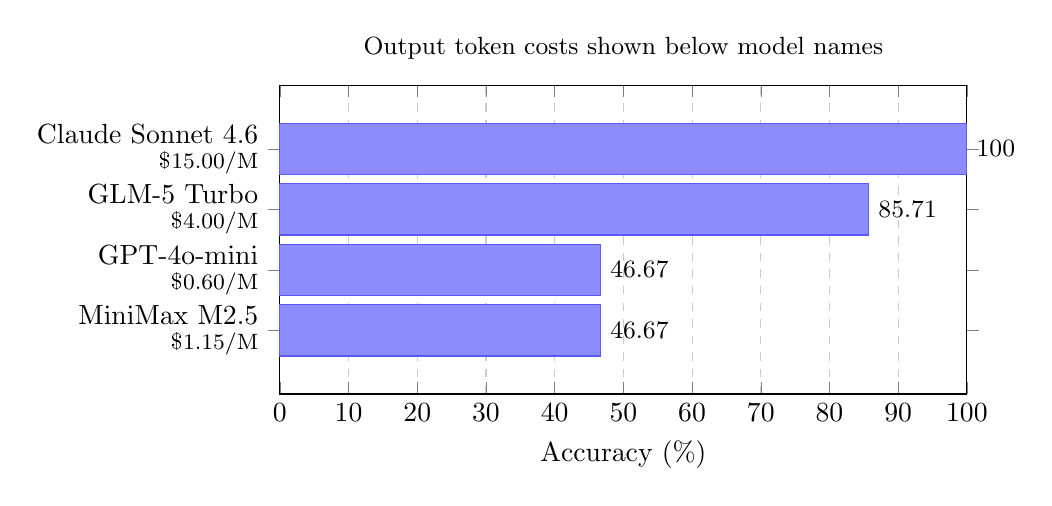
\begin{tikzpicture}
            \begin{axis}[
                xbar,
                bar width=0.65cm,
                width=0.85\linewidth,
                height=5.5cm,
                enlarge y limits=0.35,
                xlabel={Accuracy (\%)},
                xmin=0, xmax=100,
                clip=false,
                symbolic y coords={MiniMax M2.5, GPT-4o-mini, GLM-5 Turbo, Claude Sonnet 4.6},
                ytick=data,
                yticklabels={
                    {\shortstack[r]{MiniMax M2.5\\\footnotesize\$1.15/M}},
                    {\shortstack[r]{GPT-4o-mini\\\footnotesize\$0.60/M}},
                    {\shortstack[r]{GLM-5 Turbo\\\footnotesize\$4.00/M}},
                    {\shortstack[r]{Claude Sonnet 4.6\\\footnotesize\$15.00/M}}
                },
                yticklabel style={align=right},
                title={\small Output token costs shown below model names},
                nodes near coords,
                nodes near coords align={horizontal},
                nodes near coords style={font=\small},
                xmajorgrids=true,
                grid style={dashed, gray!40},
            ]
            \addplot[fill=blue!45, draw=blue!65] coordinates {
                (46.67,MiniMax M2.5)
                (46.67,GPT-4o-mini)
                (85.71,GLM-5 Turbo)
                (100,Claude Sonnet 4.6)
            };
            \end{axis}
        \end{tikzpicture}
        \caption{Tagging accuracy by model on the first prompt version.}
        \label{fig:model-accuracy}
    \end{figure}


	{\color{red}
		This section should describe the actual LLM decisions made in the project. In particular, it should explain:
		\begin{itemize}
			\item which model or models were tested or selected
			\item why those models were chosen
			\item whether the project used prompting only, fine-tuning, retrieval, or some hybrid approach
			\item how prompts were refined over time
			\item what failure cases were observed during prompt iteration
			\item how output quality was evaluated
			\item what tradeoffs were considered between model power, latency, and cost
			\item whether a smaller or cheaper model was sufficient for some subtasks
			\item whether different models were used for different stages, such as tagging, rationale generation, or scoring
			\item how hallucination risk, overflagging, and underflagging were managed
		\end{itemize}
		
		This section should also explain whether the system used fixed tag instructions, versioned prompt templates, few-shot examples, or any structured output format. If there was a decision not to fine-tune, this section should state why. If fine-tuning was considered, it should explain what training data would be needed and what risks or costs would be associated with that approach.
	}
	
	\subsection{Prompt Quality and Reviewability}

    Our prompts were refined over time to meet our stakeholders' original vision of the tagging behavior.
    For instance, one of our tags (Privacy Risk), had to be continuously refined, since the LLM was incorrectly flagging coaches who were sharing official ministry resources.

    \begin{figure}[htbp]
        \centering
        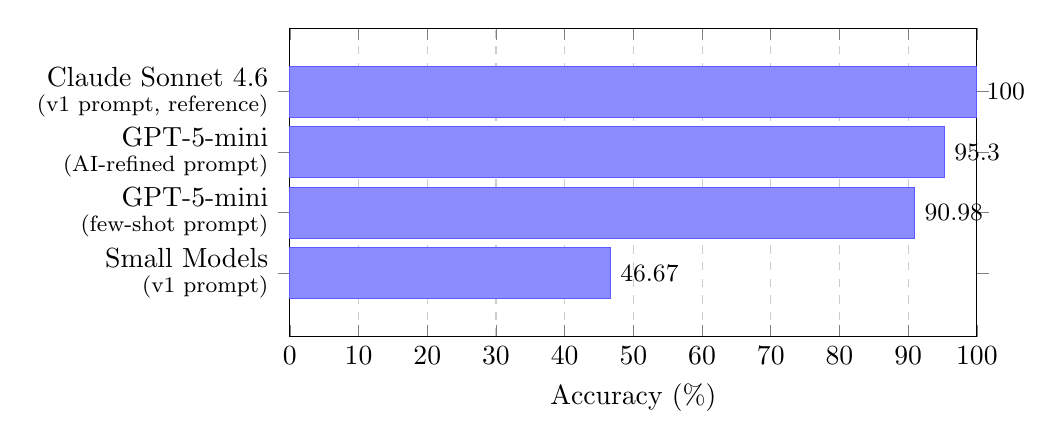
\begin{tikzpicture}
            \begin{axis}[
                xbar,
                bar width=0.65cm,
                width=0.85\linewidth,
                height=5.5cm,
                enlarge y limits=0.35,
                xlabel={Accuracy (\%)},
                xmin=0, xmax=100,
                clip=false,
                symbolic y coords={small,gpt5few,gpt5ai,claude},
                ytick=data,
                yticklabels={
                    {\shortstack[r]{Small Models\\\footnotesize(v1 prompt)}},
                    {\shortstack[r]{GPT-5-mini\\\footnotesize(few-shot prompt)}},
                    {\shortstack[r]{GPT-5-mini\\\footnotesize(AI-refined prompt)}},
                    {\shortstack[r]{Claude Sonnet 4.6\\\footnotesize(v1 prompt, reference)}}
                },
                yticklabel style={align=right},
                nodes near coords,
                nodes near coords align={horizontal},
                nodes near coords style={font=\small},
                xmajorgrids=true,
                grid style={dashed, gray!40},
            ]
            \addplot[fill=blue!45, draw=blue!65] coordinates {
                (46.67,small)
                (90.98,gpt5few)
                (95.30,gpt5ai)
                (100,claude)
            };
            \end{axis}
        \end{tikzpicture}
        \caption{Effect of prompt refinement on accuracy. GPT-5-mini (\$2.00/M output) with an AI-refined prompt reaches 95.30\%, approaching Claude Sonnet 4.6 (\$15.00/M output) at 100\% on the naive first prompt.}
        \label{fig:prompt-refinement}
    \end{figure}

	{\color{red}
		This section should explain how prompt refinement affected system behavior in practice. Good topics include:
		\begin{itemize}
			\item examples of prompts becoming more specific over time
			\item how rationale quality changed after refinement
			\item whether tags became too broad or too narrow
			\item whether score normalization or label simplification changed prompt behavior
			\item how human reviewer feedback informed prompt revisions
		\end{itemize}
	}
	
	\section{Human-in-the-Loop Review as a Design Principle}
	
	One of the strongest decisions in this project was to preserve the role of the human reviewer throughout the system design. The goal was never simply to generate tags automatically. Instead, the project aimed to build a review platform in which machine outputs could be inspected, questioned, corrected, and documented.
	
	Several features reflect this principle:
	\begin{itemize}
		\item conversation-level review status
		\item reviewer notes
		\item relevant transcript snippets linked to tags
		\item full transcript viewing
		\item false-tag feedback with required explanation
		\item reporting views that summarize outcomes without hiding raw review context
	\end{itemize}
	
	This approach matters because evaluation systems are only useful if reviewers trust them. Trust is improved when the user can see why something was flagged, inspect the source transcript, and record disagreement when necessary.
	
	\section{Challenges and Lessons Learned}
	
	A major challenge in this project was that many features crossed the frontend-backend boundary. Review status, notes, false-tag feedback, reporting, and authentication all required both interface work and backend persistence or validation. This increased integration complexity, but it also made clear that a review platform cannot be designed effectively by thinking about the frontend alone.
	
	Another challenge involved authentication. Login flow, route protection, redirect behavior, local emulation, and production configuration all had to agree on the same model. Seemingly small mismatches in request origin or runtime assumptions could produce redirect loops or invalid auth behavior. This reinforced the importance of treating authentication as a system-wide concern rather than a single frontend feature.
	
	The project also highlighted the importance of workflow-oriented design. Bugs involving pagination reset, transcript ordering, and merge drift were not merely cosmetic issues. They directly affected reviewer trust and efficiency. The system became more robust as those operational details were corrected.
	
	Finally, the architecture made clear that machine evaluation is only part of the problem. The quality of the surrounding review environment is just as important as the quality of the model output itself.
	
	\section{Future Work}
	
	Several areas remain for future work. First, the reporting interface can be expanded with additional filters, trend views, and cross-cutting breakdowns based on reviewer needs. The current reporting system is a strong foundation, but more detailed insight could improve operational oversight.
	
	Second, the LLM evaluation process itself can continue to evolve. Prompt design, scoring logic, and model selection can all be refined as more human feedback and production data become available.
	
	\section{Conclusion}
	
	This project produced a full-stack conversation review platform that combines human oversight with machine-assisted evaluation. The frontend was designed to support real reviewer tasks rather than merely display model output. The backend was designed to persist review state, support analytics, and expose structured APIs. The data model was refined to distinguish between machine-evaluation artifacts and human-review decisions, which is essential for operational clarity.
	
	Most importantly, the project demonstrates that effective LLM-assisted systems require more than just model calls. They require careful architectural decisions, transparent review workflows, usable interfaces, secure authentication, and a data model that supports correction and accountability. By combining these elements, the system moves toward a practical and extensible approach for reviewing coaching conversations at scale.
	
\end{document}
